\documentclass[parskip=full]{scrartcl}

\usepackage{amsmath}
\usepackage{hyperref}
\usepackage{graphicx}
\usepackage{subcaption}
\graphicspath {{images/}}
\hypersetup{
    colorlinks=true,
    citecolor=blue
}

\renewcommand\thesubsection{\thesection.\alph{subsection}}


\begin{document}


\title{CS698 - Assignment 3}
\subtitle{Winter 2017}
\author{
    Vineet John\\
    \texttt{v2john@uwaterloo.ca}
}
\date{\today}
\maketitle


\section{Gaussian Kernel Derivation} % (fold)
\label{sec:gaussian_kernel_derivation}

    \subsection*{Objective} % (fold)
    \label{sub:objective_1}
        Prove that the Gaussian kernel can be expressed as the inner product on an infinite dimensional feature space
        \begin{equation} \label{eqn:objective}
            k(x, x\prime) = e^{\frac{- {\lVert x - x\prime \rVert}^2}{2\sigma^2}}
        \end{equation}

    % subsection objective_1 (end)

    \subsection*{Proof} % (fold)
    \label{sub:proof_1}

        Expanding the exponent term in equation \ref{eqn:objective}, we get
        $$k(x, x\prime) = e^{\frac{-(x^Tx - 2x^Tx\prime + x\prime^Tx\prime)}{2\sigma^2}}$$

        Separating the exponent terms
        $$k(x, x\prime) = e^{\frac{-x^Tx}{2\sigma^2}} e^{\frac{x^Tx\prime}{\sigma^2}} e^{\frac{- x\prime^Tx\prime)}{2\sigma^2}}$$

        which can be written in general terms as
        \begin{equation} \label{eqn:k1_derivation}
            k(x, x\prime) = f(x) k_1(x, x\prime) f(x\prime)
        \end{equation}

        From equation \ref{eqn:k1_derivation}, we can say that
        $$k_1(x, x\prime) = e^{\frac{x^Tx\prime}{\sigma^2}} $$

        We can also write this kernel as 
        \begin{equation} \label{eqn:k2_derivation}
            k_1(x, x\prime) = e^{k_2(x, x\prime)}
        \end{equation}

        From equation \ref{eqn:k2_derivation}, we can say that
        $$k_2(x, x\prime) = \frac{x^Tx\prime}{\sigma^2}$$

        This can be further generalized as a kernel representation such that
        \begin{equation} \label{eqn:k3_derivation}
            k_2(x, x\prime) = c k_3(x, x\prime)
        \end{equation}
        where $c$ is a constant term. Here $c = \frac{1}{\sigma^2}$

        From equation \ref{eqn:k3_derivation}, we can say that
        $$k_3(x, x\prime) = x^Tx\prime$$
        which is the formulation of the identity kernel. It comprises an inner product of an input sample $x$ with another arbitrary input sample $x\prime$.

        This kernel $k_3(x, x\prime)$ can also be modified to be written as 
        \begin{equation}
            \boxed{
                k_3(x, x\prime) = \phi(x)^T\phi(x\prime)
            }
        \end{equation}
        where $\phi$ represents a mapping of the original input feature $x$ into an infinite dimensional feature space.

        Hence, it has been proved that the Gaussian kernel can be expressed as the inner product on an infinite dimensional feature space.
    
    % subsection proof_1 (end)

% section gaussian_kernel_derivation (end)


\newpage


\section{Perceptron Learning Algorithm - Dual Formulation} % (fold)
\label{sec:perceptron_learning_algorithm_dual_formulation}

    \subsection*{Objective} % (fold)
    \label{sub:objective_2}

        Given the perceptron learning rule:
        \begin{equation} \label{eqn:orig_perceptron_learning_rule}
            w^{t+1} = 
            \begin{cases}
                w^t + y_n \phi(x_n) & \text{if } y_n w^T \phi(x_n) \leq 0 \\
                w^t                 & \text{otherwise}
            \end{cases}
        \end{equation}
        show that the learned weight vector $w$ can be written as a linear combination of the vectors $y_n \phi(x_n)$ where $y_n \in \{+1, -1\}$. Denote the coefficients of this linear combination by $a_n$.

        \subsubsection*{1. Dual Formulation Objective} % (fold)
        \label{ssub:dual_formulation_objective}

            Derive a formulation of the perceptron learning rule in terms of $a_n$. Show that the feature vector $\phi(x)$ enters only in the form of the kernel function $k(x, x\prime) = \phi(x)^T\phi(x\prime)$
        
        % subsubsection dual_formulation_objective (end)

        \subsubsection*{2. Predictive Learning Rule formulation} % (fold)
        \label{ssub:predictive_learning_rule_formulation}
        
            Derive a formulation of the predictive learning rule in terms of $a_n$
            \begin{equation*}
                y = 
                \begin{cases}
                    1  & \text{if } w^T \phi(x) > 0 \\
                    -1 & \text{otherwise}
                \end{cases}
            \end{equation*}

        % subsubsection predictive_learning_rule_formulation (end)

    % subsection objective_2 (end)


    \subsection*{Proof} % (fold)
    \label{sub:proof_2}

        The implicit assumption here is that the training data $x$ has been mapping into a higher-dimensional feature space denoted by $\phi(x)$.

        Thus, we can generalize the perceptron learning rule, such that
        \begin{equation*}
            w^{t+1} = 
            \begin{cases}
                w^t + \phi(x) & \text{if } \hat{y} = 1 \text{ and } y = -1 \\
                w^t - \phi(x) & \text{if } \hat{y} = -1 \text{ and } y = 1 \\
                w^t & \text{otherwise}
            \end{cases}
        \end{equation*}
        where $\hat{y}$ is the prediction and $y$ is the target value.

        This can be further generalized to express the final weight vector after $N$ training epochs as,
        $$w = \sum_{n=1}^N y_n \phi(x_n), \forall \text{ misclassifications}$$
        which can also be written as
        \begin{equation} \label{eqn:misclassified_count}
            w = \sum_{n=1}^N a_n y_n \phi(x_n)
        \end{equation}
        where $a_n$ is the number of times $x_n$ was misclassified during the training phase. This is the only co-efficient of the linear combination equating the weight vector to $y_n \phi(x_n)$.


        Substituting the expression of $w$ obtained in equation \ref{eqn:misclassified_count} into the original perceptron learning rule denoted in equation \ref{eqn:orig_perceptron_learning_rule}, we obtain:
        \begin{equation} \label{eqn:dual_perceptron_learning_rule}
            \boxed{
                a_n = 
                \begin{cases}
                    a_n + 1 & \text{if } y_n (\sum_{n=1}^N a_n y_n) \phi(x_n)^T\phi(x_n) \leq 0 \\
                    a_n     & \text{otherwise}
                \end{cases}
            }
        \end{equation}

        Equation \ref{eqn:dual_perceptron_learning_rule} obtains the perceptron learning rule in a formulation that ensures that data only enters as an inner product term which is $\phi(x_n)^T \phi(x))$. This proves the Dual Formulation Objective(\ref{ssub:dual_formulation_objective}).


        The final prediction $y$ is obtained using the below equation
        $$y = sgn(w^T \phi(x)) $$

        Substituting the value of $w$ as obtained in equation \ref{eqn:misclassified_count}, we get
        $$y = sgn((\sum_{n=1}^N a_n y_n \phi(x_n)) \phi(x)) $$

        \begin{equation} \label{eqn:perceptron_prediction}
            \boxed{
                y = sgn(\sum_{n=1}^N a_n y_n (\phi(x_n)^T \phi(x)))            
            }
        \end{equation}

        Equation \ref{eqn:perceptron_prediction} is the formulation of the Predictive Learning Rule(\ref{ssub:predictive_learning_rule_formulation}) in terms of the co-efficient term $a_n$.
    
    % subsection proof_2 (end)

% section perceptron_learning_algorithm_dual_formulation (end)


\newpage


\section{Non-linear Regression Techniques} % (fold)
\label{sec:non_linear_regression_techniques}

    \subsection{Regularized Generalized Linear Regression} % (fold)
    \label{sub:regularized_generalized_linear_regression}
    
        Figure \ref{fig:rglg_err_v_deg} shows how the model error varies with respect to the maximum degree of basis functions. 

        \begin{figure}
            \centering
            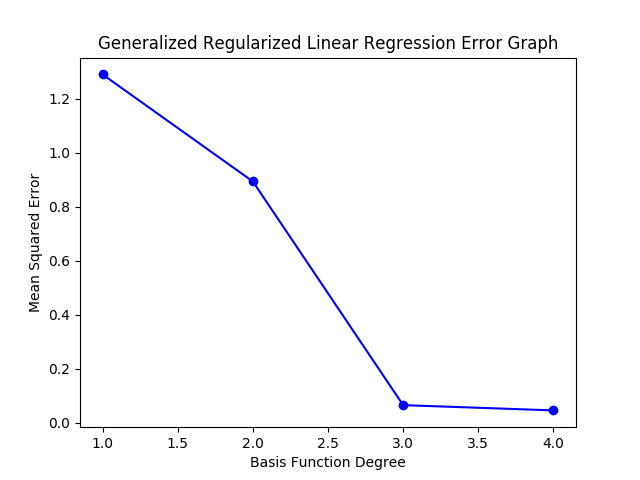
\includegraphics[width=0.7\textwidth]{3a_degree_vs_error.png}
            \caption{Regularized Generalized Linear Regression - Error vs Basis function degree}
            \label{fig:rglg_err_v_deg}
        \end{figure}

        Similarly, Figure \ref{fig:rglg_time_v_deg} shows the variation of time required for the computation as a function of the maximum basis function degree. 

        \begin{figure}
            \centering
            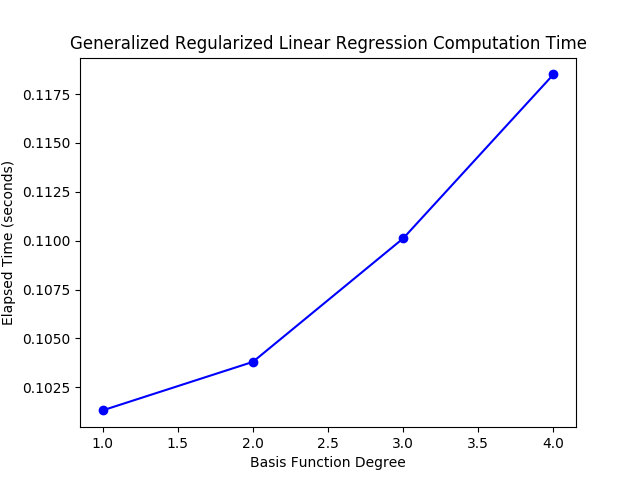
\includegraphics[width=0.7\textwidth]{3a_degree_vs_time.png}
            \caption{Regularized Generalized Linear Regression - Time vs Basis function degree}
            \label{fig:rglg_time_v_deg}
        \end{figure}

        \subsubsection*{Regularized Generalized Linear Regression - Results Discussion} % (fold)
        \label{ssub:regularized_generalized_linear_regression_results_discussion}

            The best performing basis function in terms of error minimization is the one with degree 4.

            The experiments for computational time might not be very indicative of the complexity increase, due to the low amount of time it takes to execute, but the computation seems to be increasing monotonically for increased maximum degree of basis functions. This could be attributed to the increase of the size of the weights that need to be computed, because each `n' degree basis function is a subset of any `m' degree basis function $\forall m > n$.
        
        % subsubsection regularized_generalized_linear_regression_results_discussion (end)

        The code for Regularized Generalized Linear Regression is present in the directory `regularized-generalized-linear-regression' of the code archive submitted. All the statistics reported were derived using 10-fold cross-validation.

    % subsection regularized_generalized_linear_regression (end)

    \subsection{Bayesian Generalized Linear Regression} % (fold)
    \label{sub:bayesian_generalized_linear_regression}
    
        Figure \ref{fig:bglg_err_v_deg} shows how the model error varies with respect to the maximum degree of basis functions.

        \begin{figure}
            \centering
            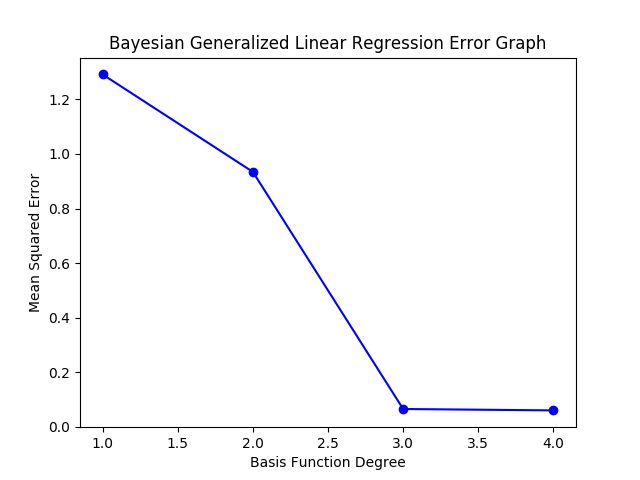
\includegraphics[width=0.7\textwidth]{3b_degree_vs_error.png}
            \caption{Bayesian Generalized Linear Regression - Error vs Basis function degree}
            \label{fig:bglg_err_v_deg}
        \end{figure}

        Figure \ref{fig:bglg_time_v_deg} shows the variation of time required for the computation as a function of the maximum basis function degree.

        \begin{figure}
            \centering
            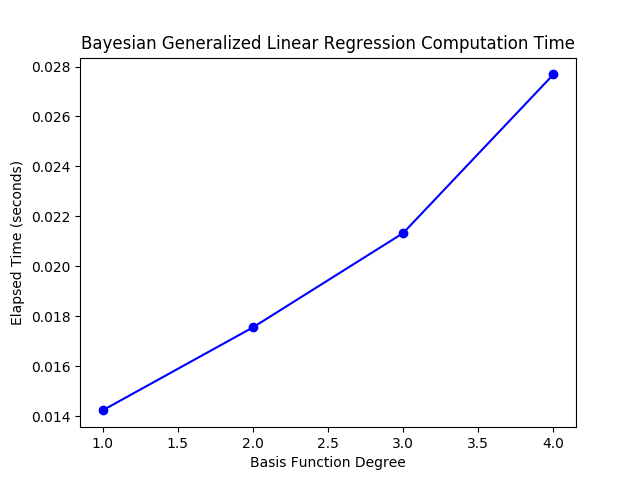
\includegraphics[width=0.7\textwidth]{3b_degree_vs_time.png}
            \caption{Bayesian Generalized Linear Regression - Time vs Basis function degree}
            \label{fig:bglg_time_v_deg}
        \end{figure}

        \subsubsection*{Bayesian Generalized Linear Regression - Results Discussion} % (fold)
        \label{ssub:bayesian_generalized_linear_regression_results_discussion}

            Similar to the previous experiment[\ref{sub:regularized_generalized_linear_regression}], the best performing basis function in terms of error minimization is the one with degree 4.

            The patterns for time complexity are also similar to those detected for Regularized Generalized Linear Regression. 
        
        % subsubsection bayesian_generalized_linear_regression_results_discussion (end)

        \subsubsection*{Regularized generalized linear regression vs. Bayesian generalized linear regression} % (fold)
        \label{ssub:regularized_generalized_linear_regression_vs_bayesian_generalized_linear_regression}

            The generalized version of linear regression allows a mapping into a higher dimensional feature space which can be utilized to perform linear regression to predict underlying functions are are non-linear. This approach is common to both Regularized generalized linear regression and Bayesian generalized linear regression.

            The difference between the two models is that Bayesian linear regression models the weight parameter as a Gaussian distribution. This leads to modeling the Bayesian linear objective's target variable as a conjugate distribution. This is because both the prior and likelihood probability distributions are Gaussian, which implicity models the target variable distribution as a Gaussian, too. This is different from regularized generalized linear regression, as for the latter, we simply obtain the solution by minimizing a convex optimization objective. However, for bayesian generalized linear regression, we iteratively minimize the search space for the ideal weights by using the computed posterior of each data-point as a prior for the next expression, thus minimizing the risk of overfitting better than simple generalized linear models.
        
        % subsubsection regularized_generalized_linear_regression_vs_bayesian_generalized_linear_regression (end)

        The code for Bayesian Generalized Linear Regression is present in the directory `bayesian-generalized-linear-regression' of the code archive submitted. All the statistics reported were derived using 10-fold cross-validation.
    
    % subsection bayesian_generalized_linear_regression (end)

    \subsection{Gaussian Process Regression} % (fold)
    \label{sub:gaussian_process_regression}

        The Gaussian process regression experiments were done on the identity, gaussian and polynomial kernels, each discussed in greater detail in the below sections.

        \subsubsection*{Identity Kernel} % (fold)
        \label{ssub:identity_kernel}

        The mean squared error obtained by 10-fold cross-validation is:
        $$MSE = 3.576$$
        The time taken for this computation was $1.185$ seconds
        
        % subsubsection identity_kernel (end)

        \subsubsection*{Gaussian Kernel} % (fold)
        \label{ssub:gaussian_kernel}

            Figure \ref{fig:gpr_gaussian_stddev_vs_error} shows how the model error varies with the standard deviation ($\sigma$) of the Gaussian distribution encoded in the kernel.

            \begin{figure}
                \centering
                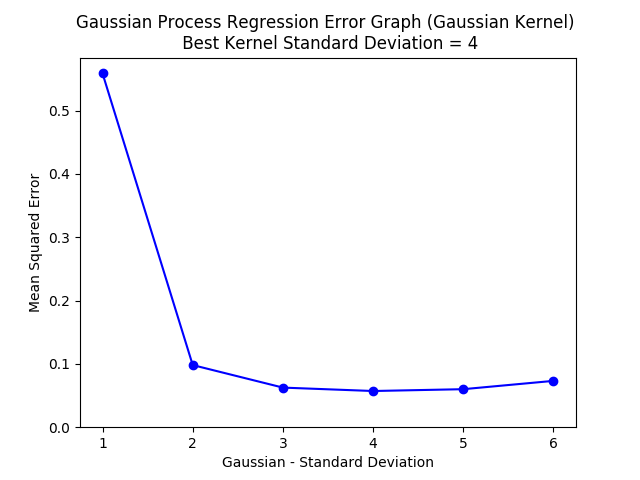
\includegraphics[width=0.7\textwidth]{3c_gpr_gaussian_stddev_vs_error.png}
                \caption{Gaussian Process Regression - Gaussian Kernel - Standard Deviation vs. Error}
                \label{fig:gpr_gaussian_stddev_vs_error}
            \end{figure}

            Figure \ref{fig:gpr_gaussian_stddev_vs_time} shows how the time complexity varies with the standard deviation ($\sigma$) of the Gaussian distribution encoded in the kernel.

            \begin{figure}
                \centering
                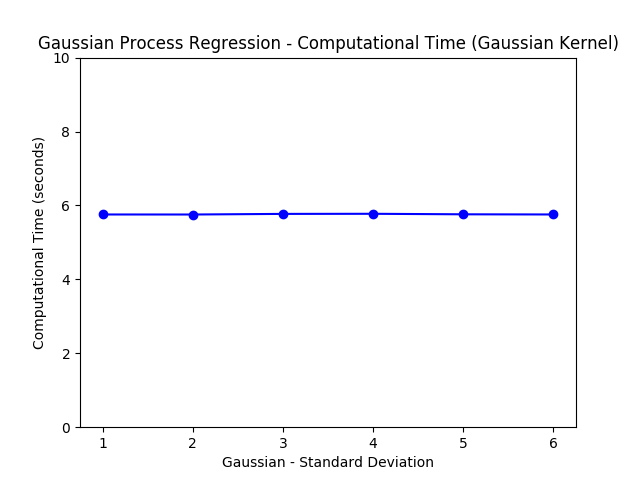
\includegraphics[width=0.7\textwidth]{3c_gpr_gaussian_stddev_vs_time.png}
                \caption{Gaussian Process Regression - Gaussian Kernel - Standard Deviation vs. Time}
                \label{fig:gpr_gaussian_stddev_vs_time}
            \end{figure}
        
        % subsubsection gaussian_kernel (end)

        \subsubsection*{Polynomial Kernel} % (fold)
        \label{ssub:polynomial_kernel}

            Figure \ref{fig:gpr_polynomial_degree_vs_error} shows how the model error varies with the polynomial degree ($d$) of the polynomial function encoded in the kernel.

            \begin{figure}
                \centering
                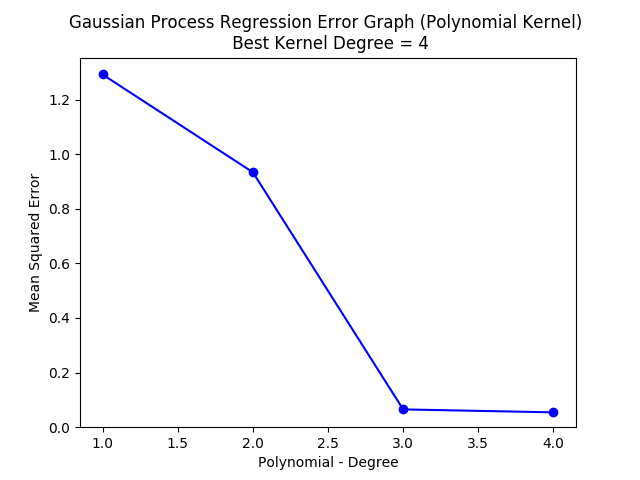
\includegraphics[width=0.7\textwidth]{3c_gpr_polynomial_degree_vs_error.png}
                \caption{Gaussian Process Regression - Polynomial Kernel - Degree vs. Error}
                \label{fig:gpr_polynomial_degree_vs_error}
            \end{figure}

            Figure \ref{fig:gpr_polynomial_degree_vs_time} shows how the time complexity varies with the polynomial degree ($d$) of the polynomial function encoded in the kernel.

            \begin{figure}
                \centering
                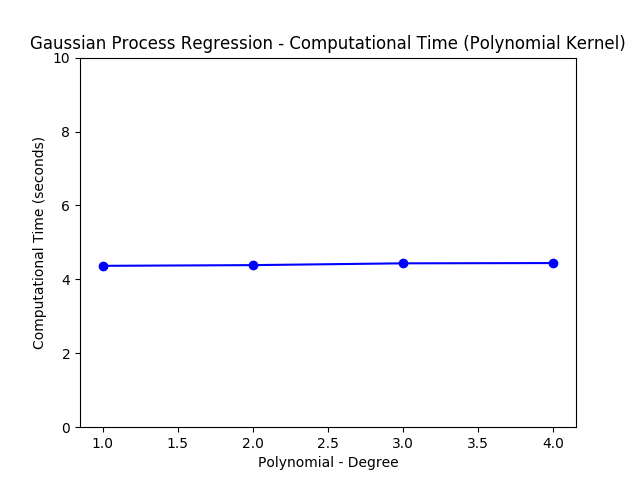
\includegraphics[width=0.7\textwidth]{3c_gpr_polynomial_degree_vs_time.png}
                \caption{Gaussian Process Regression - Polynomial Kernel - Degree vs. Time}
                \label{fig:gpr_polynomial_degree_vs_time}
            \end{figure}
        
        % subsubsection polynomial_kernel (end)

        \subsubsection*{Gaussian Process Regression - Results Discusssion} % (fold)
        \label{ssub:gaussian_process_regression_results_discusssion}

            Both the Gaussian and the Polynomial kernels obtain far better results in terms of mean squared error minimization as compared to the Identity kernel. The best mean-squared error statistic for each of the kernel implementations are given in Table \ref{tab:kernel_error_comparison}.

            \begin{table}[ht]
                \centering
                \begin{tabular}{| l | c |}
                \hline
                \textbf{Kernel} & \textbf{Best MSE} \\
                \hline
                \hline
                    Identity & 3.576 \\
                \hline
                    Gaussian & 0.057 \\
                \hline
                    Polynomial & 0.054 \\
                \hline
                \end{tabular}
                \caption{Kernel Error Comparison}
                \label{tab:kernel_error_comparison}
            \end{table}
            The best MSE for the Gaussian kernel was achieved for $\sigma = 4$ and the best MSE for the polynomial kernel was achieved for $d = 4$

            The running times for each of the variations of the parameters for the Gaussian and Polynomial do not have significant deviations in terms of run-time, which allows computation of a regression function that scales only with the data, and not the complexity of the underlying basis function. This is indicated in Table \ref{tab:kernel_computational_time_comparison}. 

            This implicitly means that the input features could theoretically be mapped into an infinite dimensional space, with no added computational cost as long as the number of data points remains the same.
            
            \begin{table}[ht]
                \centering
                \begin{tabular}{| c | c | c |}
                \hline
                \textbf{Kernel} & \textbf{Mean Time (s.)} & \textbf{Std. Dev. Time (s.)} \\
                \hline
                \hline
                    Identity & 1.185 & - \\
                \hline
                    Gaussian & 2.574 & 0.005 \\
                \hline
                    Polynomial & 1.315 & 0.016 \\
                \hline
                \end{tabular}
                \caption{Kernel Computational Time Comparison}
                \label{tab:kernel_computational_time_comparison}
            \end{table}

        
        % subsubsection gaussian_process_regression_results_discusssion (end)

        The code for Gaussian Process Regression is present in the directory `gaussian-process-regression' of the code archive submitted. All the statistics reported were derived using 10-fold cross-validation.
    
    % subsection gaussian_process_regression (end)

% section non_linear_regression_techniques (end)


\end{document}
